\question
Как известно, «мозг» любого компьютера – это процессор, в свою очередь «мозг» любого процессора – так называемое арифметико-логическое устройство (АЛУ) – специальная схема, которой можно подать на вход 2 булевых операнда, произвести над ними нужную операцию, и получить на выходе 1 или 0. Например, это устройство может выполнить операции вида AB или A + B.

На физическом уровне всё это представляет собой микросхему, состоящую из транзисторов, в которой минимальный логический элемент представляет собой операцию И-НЕ (NAND, штрих Шеффера):

\begin{figure}[h]

\begin{minipage}[h]{0.55\linewidth}
\end{minipage}
\begin{minipage}[h]{0.45\linewidth}
\center{
\includegraphics[width=0.7\textwidth]{pic/861.png} }
\end{minipage}
\end{figure}

то же самое, что

\begin{figure}[h]

\begin{minipage}[h]{0.55\linewidth}
\end{minipage}
\begin{minipage}[h]{0.45\linewidth}
\center{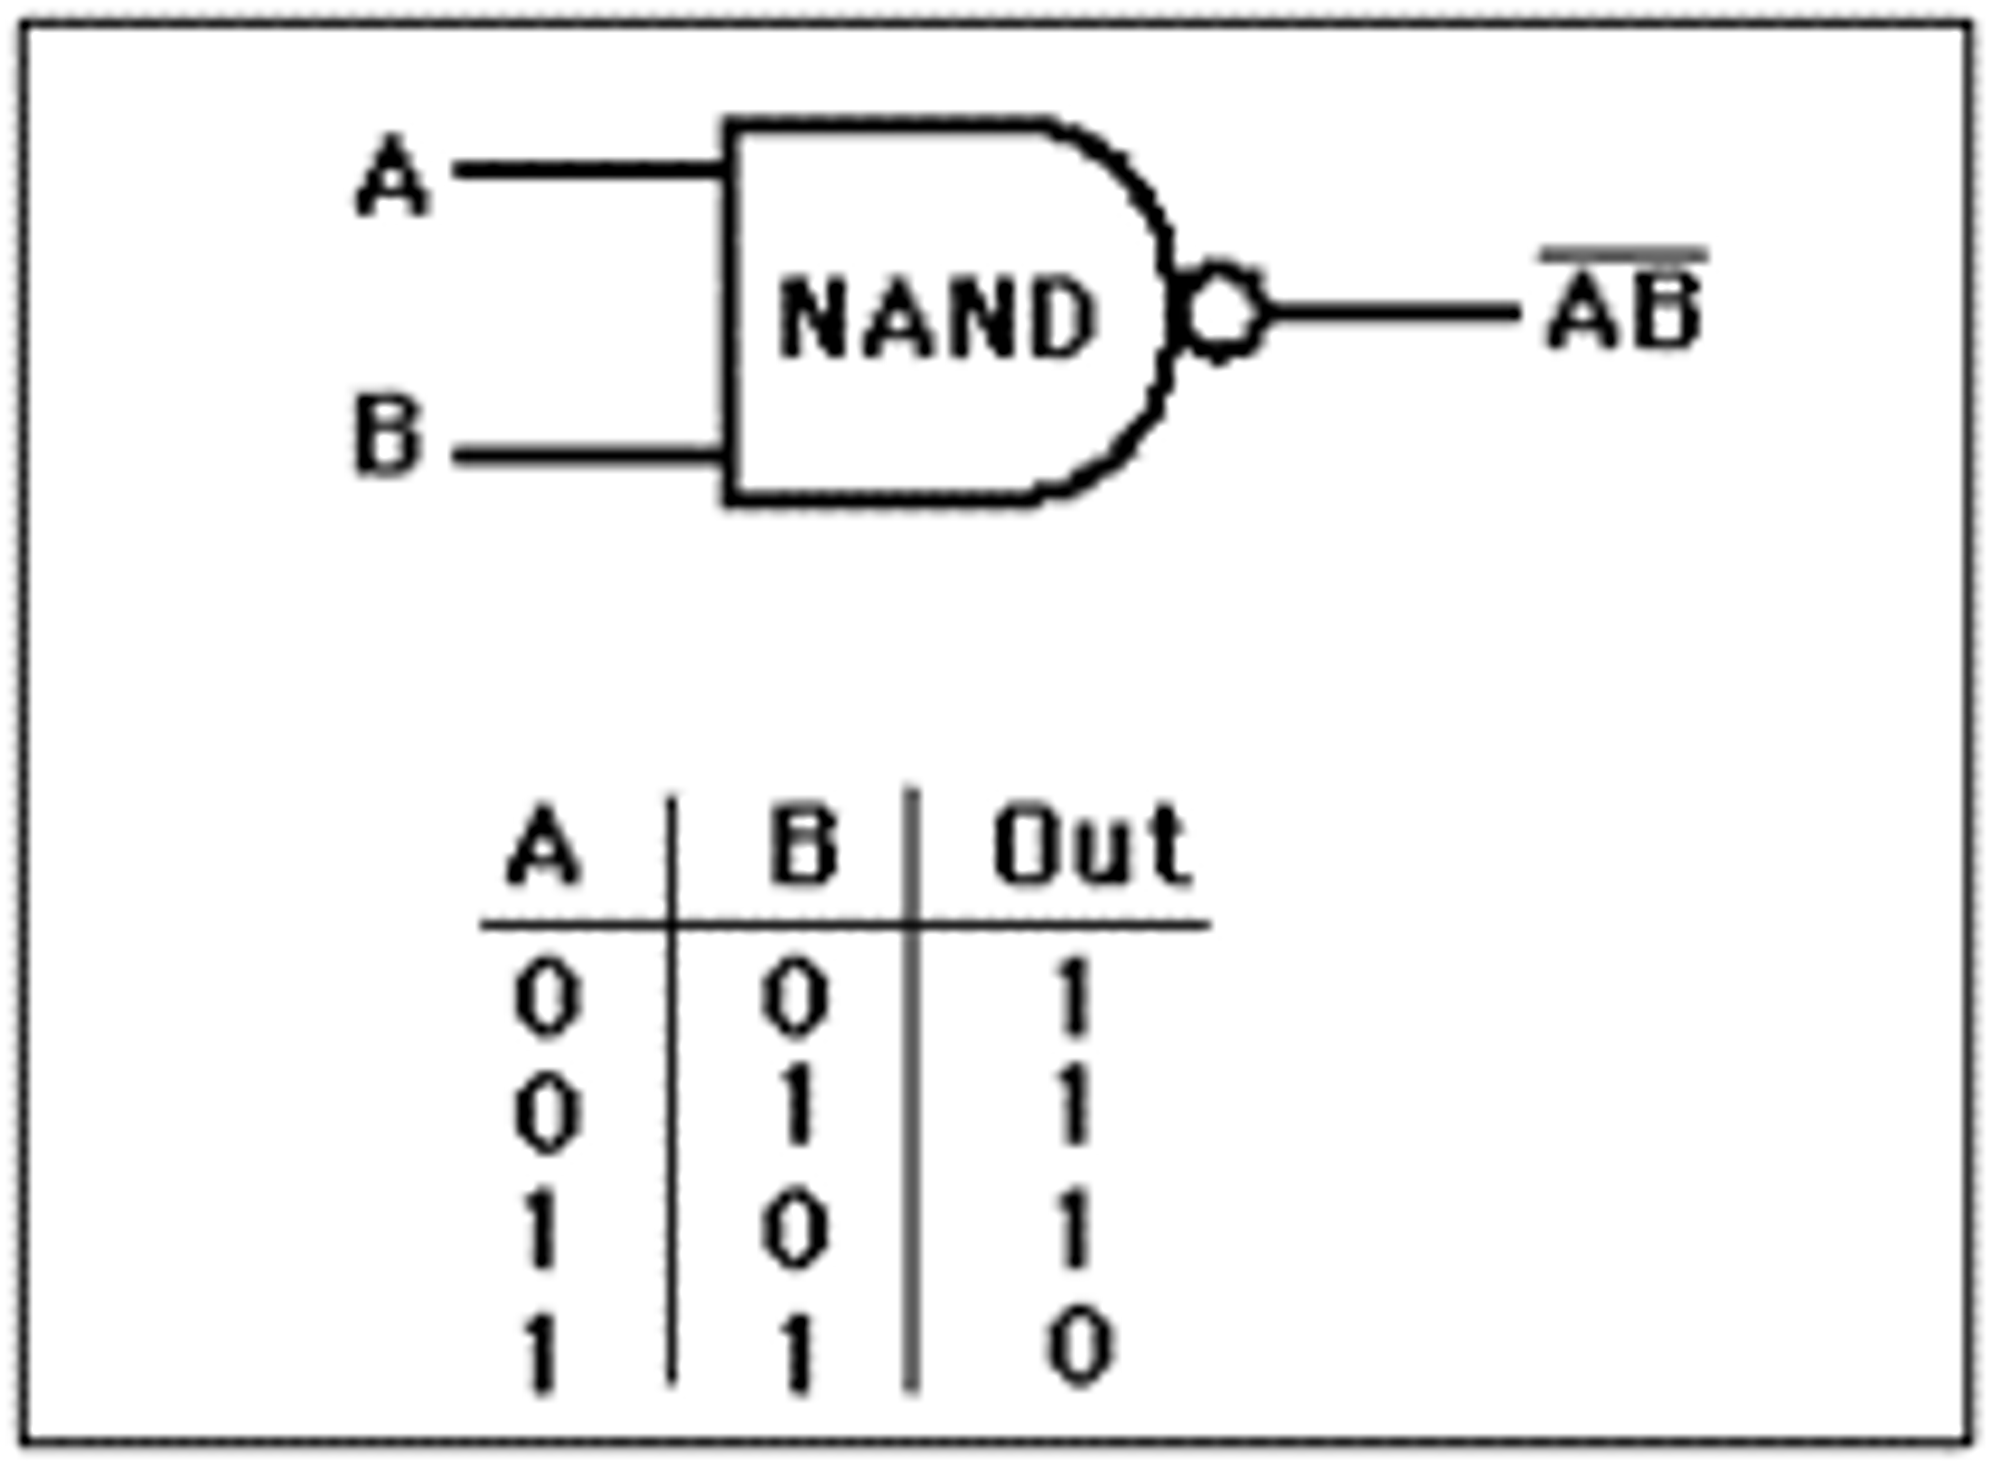
\includegraphics[width=0.7\textwidth]{pic/862.png} }
\end{minipage}
\end{figure}


Ваша задача – разработать базовый процессор. Используя только NAND, построить коммутационные схемы для простейших функций: $A \lor B$, $A \land B$, $A \oplus B$, const 1, const 0, $\neg A$, $\neg B$.

После этого, представить функцию $f(A, B, C) = \overline{A}BC + \overline{B}(C + A)$ в виде коммутационной схемы, по прежнему используя только операцию NAND.

---------------

Автор -- Тимур Гонтарь, М3206